\documentclass[../thesis.tex]{subfiles}

\begin{document}

\appendix
\renewcommand{\arraystretch}{1.25}
\section{Appendices}

\subsection{Bispherical coordinates system}
\begin{figure}[b!]
\center
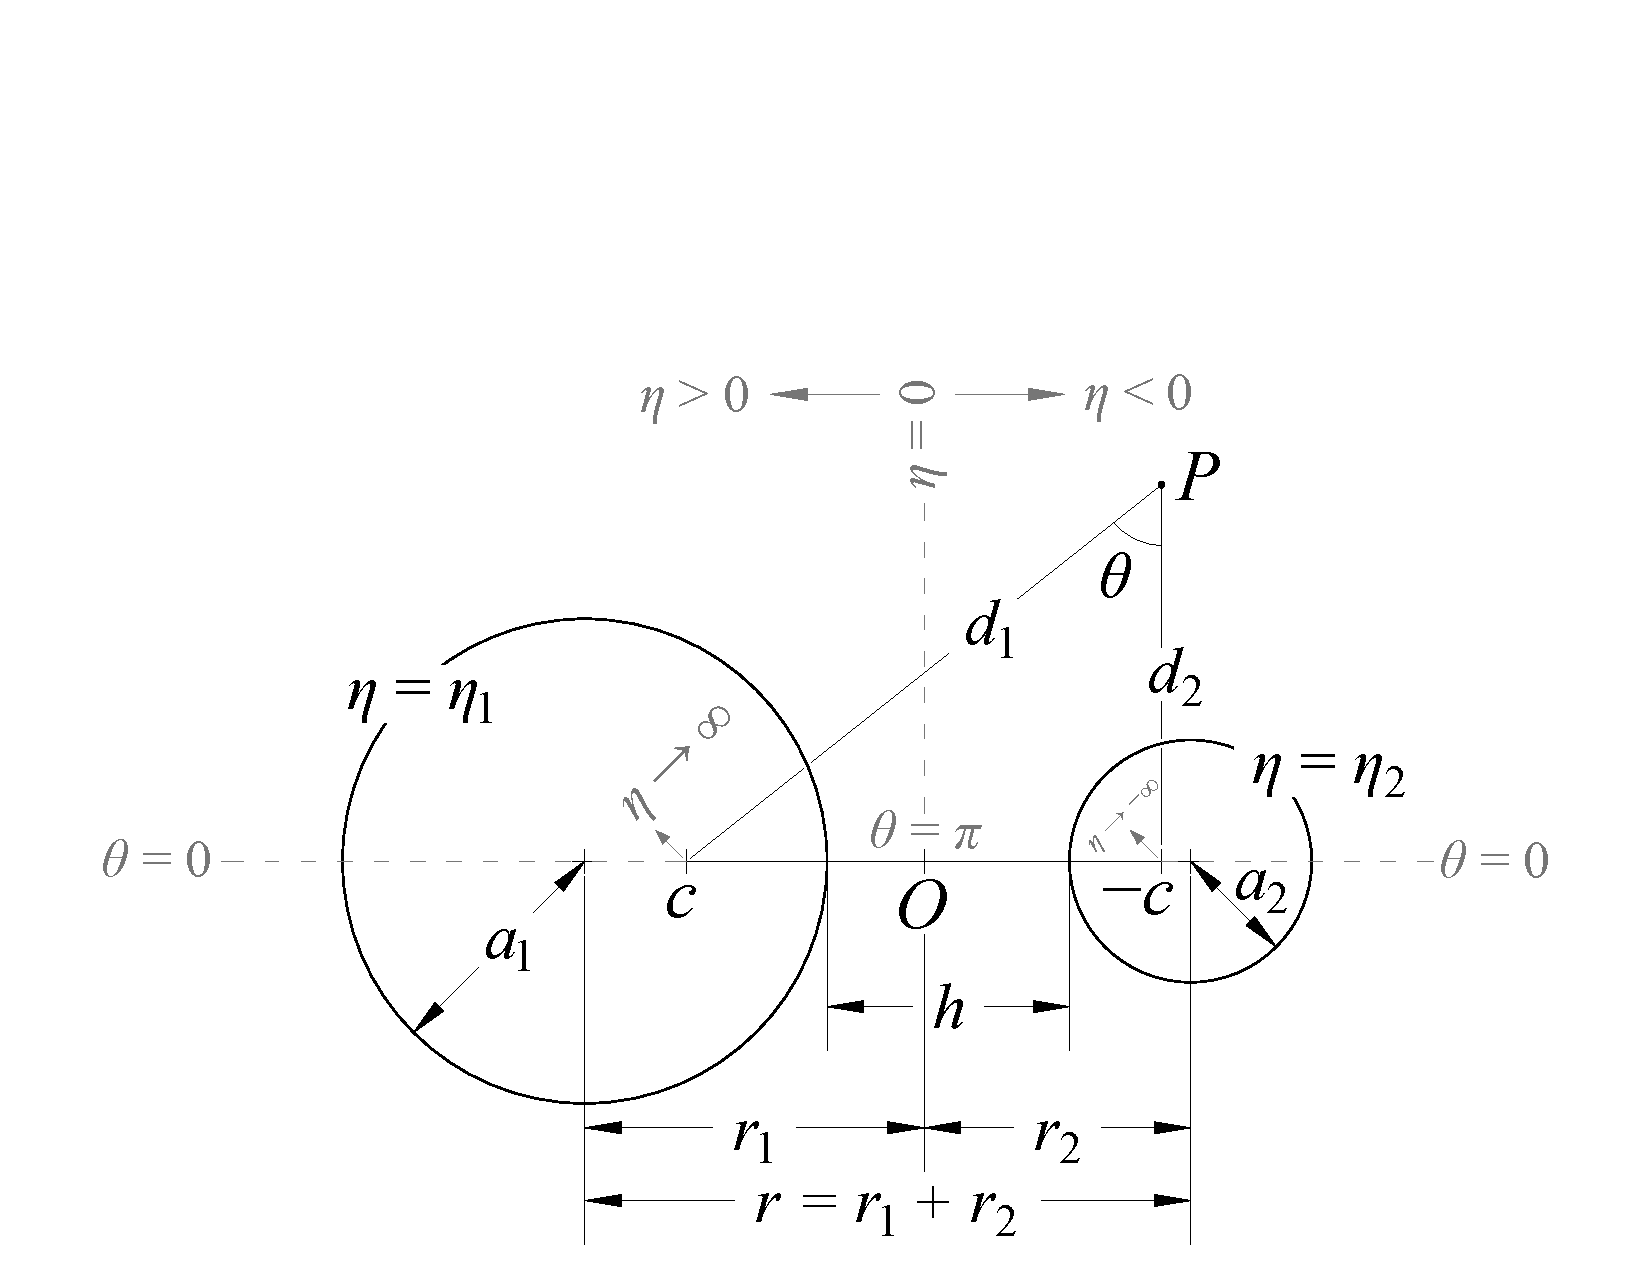
\includegraphics[trim=15mm 05mm 15mm 60mm, clip, width=0.7\textwidth]{./figs/bispherical.pdf}
\caption{Geometrical parameters for two spheres in bispherical coordinates}
\label{fig:bispherical}
\end{figure}
In Figure~\ref{fig:bispherical}, for an arbitrarily located point $P(\eta,\theta)$ the bispherical coordinates are $\eta\equiv\ln(d_2/d_1)$ and $\theta$ being the angle $P$ makes with the two focal points at $\pm c$ where
\begin{eqnarray}
c = \frac{1}{2r}\sqrt{[r^2-(a_1+a_2)^2][r^2-(a_1-a_2)^2]}.\nonumber
\end{eqnarray}
The rest of the parameters displayed in Figure~\ref{fig:bispherical} describe a distinct setting for two arbitrary spheres $\eta_1$ and $\eta_2$ whose relation with the given geometrical parameters are as follows:
\begin{align}
\sinh\eta_1 &= \frac{c}{a_1}, \qquad
\coth\eta_1 = \frac{r_1}{c}, \nonumber
\\
\sinh-\eta_2 &= \frac{c}{a_2}, \; \quad
\coth-\eta_2 = \frac{r_2}{c}, \nonumber
\\
\cosh\eta_1 &= \frac{r_1}{a_1} = 1 + \epsilon\frac{\lambda+\frac{\epsilon}{2}}{1+\lambda+\epsilon}, \label{eq:zin1}
\\
\cosh-\eta_2 &= \frac{r_2}{a_2} = 1 + \frac{\epsilon}{\lambda}\frac{1 + \frac{\epsilon}{2}}{1+\lambda+\epsilon}, \label{eq:zin2}
\end{align}
where the normalized clearance, radius ratio, and separation distance, respectively, are:
\begin{align}
\epsilon &= \frac{h}{a_1} = \xi\frac{1+\lambda}{2}, \nonumber
\\
\lambda &= \frac{a_2}{a_1} = \frac{\sinh\eta_1}{\sinh-\eta_2}, \label{eq:lam}
\\
r &= c(\coth\eta_1+\coth-\eta_2) \nonumber \\ 
  &= a_1\cosh\eta_1+a_2\cosh\eta_2 \label{eq:sep} \\ 
  &= a_1(1+\lambda+\epsilon).  \nonumber
\end{align}
For a specific two-sphere setting ($r,\lambda$), the system of Equations~(\ref{eq:lam}, \ref{eq:sep}) needs to be iteratively solved to find $(\eta_1,\eta_2)$ (see Appendix B1 of \cite{GMS20}). A better alternative is to employ explicit \cite{Z80} transforms given in (\ref{eq:zin1}, \ref{eq:zin2}). Note that due to our problem setting $\eta_2<0$, while all the rest of the geometrical and bispherical parameters are positive. Also note that $(\alpha,\beta)=(\xi_1,\xi_2)=(\eta_1,\eta_2)$ in Table~\ref{tab:misprints}. See Section IV of \cite{MS12} for more details regarding bispherical coordinates.



\subsection{Exact solutions in bispherical coordinates\label{sec:bi}}
The bispherical coordinate system has been used to solve various physical problems such as interaction of a sphere with infinite rigid or free flat surfaces \cite{B61}, interaction between two internal eccentric spheres as in a spherical journal bearing \cite{J15}, or elastic media having two spherical cavities \cite{SS52}. Here, we review relevant studies on analytical solutions for two spherical particles, both rigid and fluid, interacting through an unbounded, quiescent, viscous fluid.

The interaction of two spheres rotating around their line of centers has been investigated by \cite{J15}. \cite{SJ26} considered a system with the pair of particles translating in the same direction along their line of centers, i.e.\ following each other. In turn, \cite{M61} developed a solution of the Stokes equation, for two rigid spheres either approaching or retreating along the line of centers. \cite{B61} derived the same force representation for a sphere approaching a \textit{free} plane surface. He also showed that omission of inertial terms from N--S equations, i.e.\ Stokes regime, counterintuitively leads to having the same magnitude in force whether the sphere moves towards or away from the plane.

\cite{GCB66} solved the symmetrical (flow around two equal-sized spheres) coupled problem of a pair of particles moving in the same direction and rotating with opposite angular velocities around central axes perpendicular to their line of centers. \cite{ON69} found solutions to two problems with boundary conditions complementary to that of \cite{GCB66}, namely a pair of spheres translating in opposite directions and rotating with the same angular velocities about axes perpendicular to the line connecting their centers. These solutions require solving a system of equations for a series of decaying recurrent coefficients. \cite{ONM70} generalized this solution to the case of the asymmetric configuration with unequal-sized particles. These studies provide an exact representation of interaction between two \textit{rigid} spheres in a viscous fluid. 

By solving the Stokes flow inside the spherical particles, \cite{WW72} developed exact solutions for two identical liquid spheres following each other. They also showed that their solution in the limit of very large viscosity ratios approaches the  solution by \cite{SJ26}. This is the case of an extremely viscous internal circulation compared to the external flow. \cite{HHS73} generalized the solution to two fluid drops with different sizes and viscosities moving with any orientation along their line of centers. \cite{Z80} derived the solution for two fluid drops translating normal to that line. These studies provide a complete description of the drag forces acting on a pair of \textit{fluid} spheres.

It has to be added that the studies mentioned above were carried out under the continuum assumption of the fluid, that is in the limit of zero Knudsen number. In the range of small Knudsen numbers, \cite{RM74} developed a solution for two rigid spheres translating along their line of centers by considering free slip boundary conditions on their surfaces. Their solution approaches those of \cite{WW72} or \cite{HHS73} in the limit of low viscosity ratio. \cite{G96} and recently \cite{RSD22} developed solutions for a pair of fluid drops having free-slip boundary conditions and moving along their line of centers. Their solutions in the limit approach those derived by \cite{RM74} as well as \cite{HHS73}. These continuum--slip force representations are valid only for small Knudsen numbers, namely $Kn < 0.1$.

\paragraph{Recovering \cite{M61} results from \cite{SJ26}}
\cite{SJ26} developed \textit{explicit} formulae to evaluate forces acting on a pair of spheres moving with the same orientation along their line of centers. An \textit{implicit} alternative is to numerically solve the system of equations (26) therein. Doing so allows us to change the boundary condition and solve the complementary problem of spheres with an opposing orientation, for which \cite{M61} developed an explicit set of analytical formulation. This is simply done by changing the boundary condition for the second sphere $\beta$: using $-V$ instead of $V$ in the factor (25) of the second and fourth lines of (26). The same is valid for other studies that provide the system of equations, such as \cite{HHS73} whose solution can be calculated either implicitly by solving the system of equations given in Appendix B therein, or explicitly by using the functions given in Appendix C therein.

\paragraph{Reciprocal identities in \cite{ONM70} and \cite{D69} solutions}
In these two studies, analytical solutions are developed for the motion of an unequal pair normal to their line of centers. They decompose the general problem into sixteen sub-problems and find the overall interaction for any arbitrary case by superposing the corresponding solutions. Table 1 in both studies present such results. Some of these sub-solutions are interrelated \cite[using the notation in][]{ONM70} as follows:
\begin{align}
k f_{22}(k, \epsilon) &= f_{22}(k^{-1}, \epsilon k^{-1}),\\
k^3 g_{12}(k, \epsilon) &= g_{12}(k^{-1}, \epsilon k^{-1}),\\
3 f_{11}(k, \epsilon) &= 4 g_{21}(k, \epsilon),\\
3 f_{11}(k^{-1}, \epsilon k^{-1}) &= 4 g_{21}(k^{-1}, \epsilon k^{-1}),\\
3k^2 f_{12}(k, \epsilon) &= 4 g_{22}(k^{-1}, \epsilon k^{-1}),\\
3 f_{12}(k^{-1}, \epsilon k^{-1}) &= 4k^2 g_{22}(k, \epsilon),
\end{align}
in which $k=\tfrac{a_2}{a_1}(=\lambda)$ and $\epsilon=\tfrac{h}{a_1}$.



\subsection{List of misprints}%misprints_misprints_misprints_misprints_misprints
Rigorous numerical test were conducted to compare the force and torque representation from twin multipole expansion method by \cite{JO84} with the solutions developed in bispherical coordinates. The comparison, showed us some of the potential misprints in all these studies, some of which already reported by others. Table~\ref{tab:misprints} lists these misprints.



\subsection{Tables of collision efficiency\label{sec:E12}}

The three Tables \ref{tab:E10}, \ref{tab:E20}, and \ref{tab:E30} provide the results of simulations performed to compute the collision efficiency of a pair of droplets settling under gravity. The same values are plotted in Figure~\ref{fig:E12}.



\begin{landscape}

\begin{longtable}{p{3cm}p{3cm}p{5.0cm}p{5.25cm}p{5.5cm}}
 \hline
 Study & Equation & Misprinted form & Corrected form & Description \\ \hline
 \cite{SJ26} & (37) & $\frac{2}{3}$ & $\frac{4}{3}$ & \cite{HB83,M61}.\\ \hline
 
 \cite{M61} & $F_1$ \& $F_2$ & $(A_n \mp B_n + C_n \mp D_n)$ & $(A_n' \pm B_n' + C_n' \pm D_n')$ & \multirow[t]{7}{5.5cm}{\cite{GMS20} provided the correct form. Also, computational tests based on cross-comparison of the factors with their counterparts in \cite{SJ26}.} \\ \cline{2-4}
 & $\Delta B_n'$ & $\big[-4\exp\left(n+\tfrac{1}{2}\right)\left(\alpha-\beta\right)$ & $\big[-4\exp\left\{-\left(n+\tfrac{1}{2}\right)\left(\alpha-\beta\right)\right\}$ & \\ 
 & & $\cdots+\cdots\cosh\left(\alpha-\beta\right)\big]$ & $\cdots+\cdots\cosh\left(\alpha+\beta\right)\big]$ & \\ \cline{2-4}
 & $\Delta C_n'$ & $\big[\cdots\sinh\left(n+\tfrac{3}{2}\right)\left(\alpha-\beta\right)$ & $\big[\cdots\sinh\left(n+\tfrac{3}{2}\right)\left(\alpha+\beta\right)$ & \\ 
 & & $- \cdots\sinh\left(n+\tfrac{1}{2}\right)\left(\alpha-\beta\right)$ & $- \cdots\sinh\left(n+\tfrac{1}{2}\right)\left(\alpha-\beta\right)$ & \\
 & & $\times\sinh\left(n+\tfrac{1}{2}\right)\left(\alpha-\beta\right) \cdots \big]$ & $\times\sinh\left(n+\tfrac{1}{2}\right)\left(\alpha+\beta\right) \cdots \big]$ & \\ \cline{2-4}
 & $\Delta D_n'$ & $\big[\cdots\sinh\left(n+\tfrac{1}{2}\right)\left(\alpha+\beta\right) \cdots \big]$ & $\big[\cdots\sinh\left(n+\tfrac{1}{2}\right)\left(\alpha-\beta\right) \cdots \big]$ &
  \\ \hline
  
 \cite{ONM70} & (5.10) & $\sinh^2|\beta|$ & $\sinh^3|\beta|$ & Torque: $G_\Omega \propto b^3$.
 \\ \hline
 
 \cite{WW72} & (2.46): last factor & $\left(2n-1\right)$ & $\left(2n+1\right)$ & \footnote{For very large viscosity ratios the solution for a fluid drop ($\sigma\to\infty$ in \cite{WW72}) approaches that of a rigid particle ($\lambda$ in \cite{SJ26}). A careful comparison at this limit shows the factor is misprinted.}\cite{SJ26}; computational tests compared with Table 1 in \cite{WW72}.
 \\ \hline
 
%%%%%%%%%%%%%%%%%%%%%%%%%%%%%%%%%%%%%%%%%%%%%%%%%%
 \multicolumn{5}{c}{(Continued on the next page)}%
 \\ \newpage \hline								 %
 Study & Equation & Misprinted form & Corrected  %
 form & Description \\ \hline					 %
%%%%%%%%%%%%%%%%%%%%%%%%%%%%%%%%%%%%%%%%%%%%%%%%%%
 
 \multirow[t]{3}{3cm}{\cite{HHS73}} & $[32]$ \& $[33]$ & $c$ & $c^2$ & \cite{Z82}; note: \mbox{$c=a\sinh(\alpha)$}.
 \\ \cline{2-5}
 & $[$C-7$]$ & $\delta_3=2(2n+1)^2$ & $\delta_3=-2(2n+1)^2$ & \cite{Z82}.
 \\ \cline{2-5}
 & $[$B-8$]$ & $-C_n^\alpha e^{(n+3/2)\alpha}$ & $+C_n^\alpha e^{-(n+3/2)\alpha}$ & Cross-comparison of the systems of equations in \cite{WW72} -- third line of (2.30) -- and in \cite{HHS73}; computational tests.
 \\ \hline
 
 \cite{RM74} & (20): last line & $\mp n(n+1)$ & $\pm n(n+1)$ & Cross-comparison with (26) in \cite{SJ26}.
 \\ \hline
 
 \cite{BRI78} & $[1]$: last line & $\Big\{\cdots-(2n-1)\sinh2\alpha]\Big\}$ & $\Big\{\cdots-(2n+1)\sinh2\alpha]\Big\}$ & Section III.C in \cite{DSR89}, Section 9.4.3 in \cite{KK13}, and $[$B-12$]$ in \cite{HHS73}.
 \\ \cline{2-4}
 & $[3]$ & $K_n=\frac{(n+1)}{(2n+2)(2n-1)}$ & $K_n=\frac{n(n+1)}{(2n+3)(2n-1)}$ &
 \\ \hline
 
 \cite{KK13} & (9.39): $N_1^{(n)}$ & $-2(2n+1)\sinh2\alpha$ & $+2(2n+1)\sinh2\alpha$ & \footnote{For very large viscosity ratios the solution for a fluid drop ($\lambda\to\infty$ in \cite{KK13}) approaches that of a rigid particle ($\lambda_2$ in \cite{M61}). A careful comparison at this limit shows the factor is misprinted.}\cite{M61}; computational tests compared with \cite{HHS73} and \cite{BRI78}.
 \\ \hline
 
%%%%%%%%%%%%%%%%%%%%%%%%%%%%%%%%%%%%%%%%%%%%%%%%%%
 \multicolumn{5}{c}{(Continued on the next page)}%
 \\ \newpage \hline								 %
 Study & Equation & Misprinted form & Corrected  %
 form & Description \\ \hline					 %
%%%%%%%%%%%%%%%%%%%%%%%%%%%%%%%%%%%%%%%%%%%%%%%%%%

 \multirow[t]{7}{3cm}{\cite{JO84}} & (4.9) & $P_{s(q-s)(p-n+1)}$ & $P_{s(q-s)(p-n-1)}$ & \cite{RWMG11,T17,I}.
 \\ \cline{2-5}
 & (6.12) & $f_{2j}$ & $f_{2k}$ & \multirow[c]{2}{5.5cm}{\cite{I}.}
 \\ \cline{2-4}
 & (6.13) & $\Big\{\cdots\frac{\lambda^2}{1+\lambda}\Big\}$ & $\underbrace{-\tfrac{16\lambda^2}{(1+\lambda)^4}}_\text{missing term}\cdots\Big\{\cdots\underbrace{\tfrac{\lambda^2}{4(1+\lambda)}}_\text{correction}\Big\}$ & 
 \\ \cline{2-5}
  & (7.10): $g_4$ & $\frac{4}{5}\frac{\lambda^2}{(1+\lambda)^4}$ & $\frac{\lambda^2}{10(1+\lambda)}$ & Table 11.5 in \cite{KK13}.
 \\ \cline{2-5}
 & \multirow[t]{3}{3cm}{(7.10): $g_5$} & \multirow[t]{3}{5.25cm}{$\frac{4}{125}\frac{\lambda(43-24\lambda+43\lambda^2)}{(1+\lambda)^4}$} & \cite{KK13}: $\frac{1}{250}\frac{\lambda(43-24\lambda+43\lambda^2)}{(1+\lambda)}$ & \multirow[t]{3}{5.5cm}{Computational tests show \cite{I} suggestion better approximates $g_{11}$ \& $g_{12}$ of \cite{ONM70}.} \\
 & & & \cite{L90}: $\frac{2}{125}\frac{\lambda(43-24\lambda+43\lambda^2)}{(1+\lambda)^4}$ & \\
 & & & \cite{I}: $\frac{1}{125}\frac{\lambda(43-24\lambda+43\lambda^2)}{(1+\lambda)^4}$ & 
 \\ \hline
 
 \cite{GMS20} & (60) & $\frac{n+1}{2n+3}$ & $\frac{n+2}{2n+3}$ & Printed correctly in (C35). Also, (3.45) in \cite{GCB66}.
 \\ \hline
 
%%%%%%%%%%%%%%%%%%%%%%%%%%%%%%%%%%%%%%%%%%%%%%%%%%
 \multicolumn{5}{c}{(Continued on the next page)}%
 \\ \newpage \hline								 %
 Study & Equation & Misprinted form & Corrected  %
 form & Description \\ \hline					 %
%%%%%%%%%%%%%%%%%%%%%%%%%%%%%%%%%%%%%%%%%%%%%%%%%% 
 
 \multirow[t]{6}{3cm}{\cite{RSD22}} & (A.11) & $e^{\frac{-(n+3/2)\eta_1}{2n+3}}-e^{\frac{-(n-1/2)\eta_1}{2n-1}}$ & $\frac{e^{-(n+3/2)\eta_1}}{2n+3}-\frac{e^{-(n-1/2)\eta_1}}{2n-1}$ & \multirow[c]{2}{5.5cm}{Printed correctly in \cite{R09}.}
 \\ \cline{2-4}
 & (A.12) & $e^{\frac{-(n+3/2)\eta_2}{2n+3}}-e^{\frac{-(n-1/2)\eta_2}{2n-1}}$ & $\frac{e^{(n+3/2)\eta_2}}{2n+3}-\frac{e^{(n-1/2)\eta_2}}{2n-1}$ & 
 \\ \cline{2-5}
 & (A.14) & $E_{n-1}e^{-(n-3/2)(\eta_2)}$ & $E_{n-1}e^{-(n-3/2)(\eta_2-\eta_1)}$ & \multirow[t]{4}{5.5cm}{Computational tests compared with \cite{HHS73} and \cite{RM74}.}
 \\ \cline{2-4}
 & (A.14) & $E_{n}e^{-(n-1/2)(\eta_2)}$ & $E_{n}e^{-(n-1/2)(\eta_2-\eta_1)}$ &
 \\ \cline{2-4}
 & (A.14) & $\frac{(n+1/2)^2 e^{-(n+1/2)\eta_2}}{2n+1}$ & $\frac{(n+1/2)^2 e^{(n+1/2)\eta_2}}{2n+1}$ &
 \\ \cline{2-4}
 & (A.15) \& (A.16) & $\boldsymbol{F_i}=-4\sqrt{2}\pi\mu_e/c \sum f(n,\eta_i)$ & $\boldsymbol{F_i}=-4\pi\mu_e c \sum f(n,\eta_i)$ &
 \\ \hline
%\end{tabular}
\caption{A list of misprints found in the studies on two-sphere problem}
\label{tab:misprints}
\end{longtable}%------------------------------------

\end{landscape}
\newgeometry{margin=2.75cm}
\begin{landscape}

\begin{longtable}{lllllllllll}%E12(10)_E12(10)_E12(10)
\captionsetup{width=1.35\textwidth}
 \hline
 $\lambda$ & \makecell[l]{ISM RP\\$\hat{\mu}_r=10^5$} & \makecell[l]{ISM FD\\$\hat{\mu}_r=10^2$} & \makecell[l]{Exact RP\\CL (JO)} & \makecell[l]{Exact RP\\CL (Bi)} & \makecell[l]{Exact RP\\NCL (JO)} & \makecell[l]{Exact RP\\+Rot.\ (JO)} & \makecell[l]{Exact RP\\+Rot.\ (Bi)} & \makecell[l]{Exact FD\\$\hat{\mu}_r=10^5$} & \makecell[l]{Exact FD\\$\hat{\mu}_r=10^2$}
 \\\hline
 0.05 & 0.001113 & 0.001569 & 0.000528 & 0.000525 & 0.003776 & 0.000478 & 0.000475 & 0.000475 & 0.000693
 \\
 & 0.001043$^*$ & 0.001494$^*$ & & & 0.003656$^*$ & & & & 0.000204$^*$
 \\
 0.1 & 0.003474 & 0.004283 & 0.001503 & 0.001503 & 0.008016 & 0.001273 & 0.001275 & 0.001272 & 0.001660
 \\
 & 0.003348$^*$ & 0.004153$^*$ & & & 0.007850$^*$ & & & & 0.000490$^*$
 \\
 0.15 & 0.006236 & 0.007327 & 0.002751 & 0.002750 & 0.012567 & 0.002199 & 0.002199 & 0.002189 & 0.002749
 \\
 & 0.006064$^*$ & 0.007151$^*$ & & & 0.012323$^*$ & & & & 0.000812$^*$
 \\
 0.2 & 0.008980 & 0.010298 & 0.004172 & 0.004179 & 0.017132 & 0.003173 & 0.003180 & 0.003158 & 0.003899
 \\
 & 0.008770$^*$ & 0.010085$^*$ & & & 0.016814$^*$ & & & & 0.001157$^*$
 \\
 0.25 & 0.011544 & 0.013048 & 0.005729 & 0.005727 & 0.021547 & 0.004184 & 0.004184 & 0.004149 & 0.005080
 \\
 & 0.011303$^*$ & 0.012803$^*$ & & & 0.021160$^*$ & & & & 0.001517$^*$
 \\
 0.3 & 0.013891 & 0.015547 & 0.007347 & 0.007338 & 0.025703 & 0.005196 & 0.005190 & 0.005142 & 0.006269
 \\
 & 0.013624$^*$ & 0.015276$^*$ & & & 0.025252$^*$ & & & & 0.001890$^*$
 \\
 0.35 & 0.016021 & 0.017804 & 0.008962 & 0.008955 & 0.029522 & 0.006181 & 0.006176 & 0.006118 & 0.007441
 \\
 & 0.015733$^*$ & 0.017512$^*$ & & & 0.029013$^*$ & & & & 0.002272$^*$
 \\
 0.4 & 0.017943 & 0.019832 & 0.010523 & 0.010523 & 0.032943 & 0.007118 & 0.007120 & 0.007056 & 0.008570
 \\
 & 0.017637$^*$ & 0.019522$^*$ & & & 0.032383$^*$ & & & & 0.002654$^*$
 \\
 0.45 & 0.019660 & 0.021638 & 0.011986 & 0.011993 & 0.035923 & 0.007990 & 0.007997 & 0.007933 & 0.009625
 \\
 & 0.019340$^*$ & 0.021313$^*$ & & & 0.035315$^*$ & & & & 0.003029$^*$
 \\
 0.5 & 0.021174 & 0.023224 & 0.013309 & 0.013320 & 0.038430 & 0.008774 & 0.008784 & 0.008725 & 0.010578
 \\
  & 0.020842$^*$ & 0.022887$^*$ & & & 0.037780$^*$ & & & & 0.003401$^*$
  
%%%%%%%%%%%%%%%%%%%%%%%%%%%%%%%%%%%%%%%%%%%%%%%%%%
 \\ \hline \multicolumn{10}{c}{(Continued on the next page)}
 \\ \newpage \hline $\lambda$ & \makecell[l]{ISM RP\\$\hat{\mu}_r=10^5$} & \makecell[l]{ISM FD\\$\hat{\mu}_r=10^2$} & \makecell[l]{Exact RP\\CL (JO)} & \makecell[l]{Exact RP\\CL (Bi)} & \makecell[l]{Exact RP\\NCL (JO)} & \makecell[l]{Exact RP\\+Rot.\ (JO)} & \makecell[l]{Exact RP\\+Rot.\ (Bi)} & \makecell[l]{Exact FD\\$\hat{\mu}_r=10^5$} & \makecell[l]{Exact FD\\$\hat{\mu}_r=10^2$}
 \\\hline
%%%%%%%%%%%%%%%%%%%%%%%%%%%%%%%%%%%%%%%%%%%%%%%%%%

 0.55 & 0.022489 & 0.024596 & 0.014457 & 0.014471 & 0.040451 & 0.009451 & 0.009463 & 0.009412 & 0.011403
 \\
 & 0.022146$^*$ & 0.024249$^*$ & & & 0.039763$^*$ & & & & 0.003675$^*$
 \\
 0.6 & 0.023616 & 0.025767 & 0.015405 & 0.015420 & 0.041987 & 0.010006 & 0.010019 & 0.009977 & 0.012083
 \\
 & 0.023265$^*$ & 0.025412$^*$ & & & 0.041265$^*$ & & & & 0.003641$^*$
 \\
 0.65 & 0.024579 & 0.026763 & 0.016140 & 0.016154 & 0.043053 & 0.010430 & 0.010441 & 0.010410 & 0.012605
 \\
 & 0.024222$^*$ & 0.026402$^*$ & & & 0.042297$^*$ & & & & 0.003985$^*$
 \\
 0.7 & 0.025417 & 0.027624 & 0.016657 & 0.016670 & 0.043672 & 0.010719 & 0.010729 & 0.010708 & 0.012966
 \\
 & 0.025056$^*$ & 0.027259$^*$ & & & 0.042886$^*$ & & & & 0.004149$^*$
 \\
 0.75 & 0.026188 & 0.028409 & 0.016962 & 0.016973 & 0.043879 & 0.010875 & 0.010884 & 0.010870 & 0.013167
 \\
 & 0.025823$^*$ & 0.028041$^*$ & & & 0.043065$^*$ & & & & 0.004246$^*$
 \\
 0.8 & 0.026966 & 0.029197 & 0.017067 & 0.017077 & 0.043716 & 0.010907 & 0.010915 & 0.010906 & 0.013220
 \\
 & 0.026597$^*$ & 0.028825$^*$ & & & 0.042874$^*$ & & & & 0.004265$^*$
 \\
 0.85 & 0.027847 & 0.030084 & 0.016992 & 0.017000 & 0.043226 & 0.010825 & 0.010832 & 0.010827 & 0.013136
 \\
 & 0.027477$^*$ & 0.029710$^*$ & & & 0.042358$^*$ & & & & 0.004224$^*$
 \\
 0.9 & 0.028948 & 0.031186 & 0.016759 & 0.016766 & 0.042458 & 0.010643 & 0.010649 & 0.010646 & 0.012934
 \\
 & 0.028576$^*$ & 0.030812$^*$ & & & 0.041564$^*$ & & & & 0.004133$^*$
 \\
 0.95 & 0.030399 & 0.032632 & 0.016394 & 0.016401 & 0.041458 & 0.010377 & 0.010382 & 0.010384 & 0.012631
 \\
 & 0.030028$^*$ & 0.032258$^*$ & & & 0.040539$^*$ & & & & 0.004000$^*$
 \\
 0.99 & 0.031904 & 0.034125 & 0.016024 & 0.016031 & 0.040524 & 0.010113 & 0.010118 & 0.010114 & 0.012329
 \\
 & 0.031535$^*$ & 0.033753$^*$ & & & 0.039585$^*$ & & & & 0.003869$^*$
 \\ \hline
 \caption{Collision efficiency between pairs of $a_1=10~\mu$m and $a_2=\lambda a_1$. Values on the first and second lines of every row are computed considering a normalized collision gap of $\xi_\text{col}=10^{-3}$ and $0$ (marked with asterisk), respectively.}
\label{tab:E10}
\end{longtable}%------------------------------------

\newpage

\begin{longtable}{lllllllllll}%E12(20)_E12(20)_E12(20)
\captionsetup{width=1.35\textwidth}
 \hline
 $\lambda$ & \makecell[l]{ISM RP\\$\hat{\mu}_r=10^5$} & \makecell[l]{ISM FD\\$\hat{\mu}_r=10^2$} & \makecell[l]{Exact RP\\CL (JO)} & \makecell[l]{Exact RP\\CL (Bi)} & \makecell[l]{Exact RP\\NCL (JO)} & \makecell[l]{Exact RP\\+Rot.\ (JO)} & \makecell[l]{Exact RP\\+Rot.\ (Bi)} & \makecell[l]{Exact FD\\$\hat{\mu}_r=10^5$} & \makecell[l]{Exact FD\\$\hat{\mu}_r=10^2$}
 \\\hline
 0.05 & 0.001016 & 0.001468 & 0.000550 & 0.000547 & 0.002446 & 0.000499 & 0.000496 & 0.000495 & 0.000721
 \\
 & 0.000947$^*$ & 0.001394$^*$ & & & 0.002347$^*$ & & & & 0.000220$^*$
 \\
 0.1 & 0.002785 & 0.003577 & 0.001728 & 0.001728 & 0.006207 & 0.001475 & 0.001476 & 0.001460 & 0.001897
 \\
 & 0.002663$^*$ & 0.003449$^*$ & & & 0.006019$^*$ & & & & 0.000577$^*$
 \\
 0.15 & 0.005087 & 0.006202 & 0.003611 & 0.003609 & 0.011288 & 0.002932 & 0.002931 & 0.002859 & 0.003570
 \\
 & 0.004915$^*$ & 0.006023$^*$ & & & 0.010995$^*$ & & & & 0.001115$^*$
 \\
 0.2 & 0.008881 & 0.010459 & 0.006370 & 0.006380 & 0.017899 & 0.004962 & 0.004973 & 0.004808 & 0.005872
 \\
 & 0.008644$^*$ & 0.010213$^*$ & & & 0.017497$^*$ & & & & 0.001892$^*$
 \\
 0.25 & 0.015892 & 0.018221 & 0.010261 & 0.010257 & 0.026271 & 0.007749 & 0.007747 & 0.007439 & 0.008987
 \\
 & 0.015555$^*$ & 0.017875$^*$ & & & 0.025749$^*$ & & & & 0.002993$^*$
 \\
 0.3 & 0.029692 & 0.033148 & 0.015433 & 0.015413 & 0.036512 & 0.011410 & 0.011394 & 0.010916 & 0.013107
 \\
 & 0.029227$^*$ & 0.032684$^*$ & & & 0.035855$^*$ & & & & 0.004513$^*$
 \\
 0.35 & 0.053900 & 0.058371 & 0.021875 & 0.021857 & 0.048407 & 0.015975 & 0.015961 & 0.015319 & 0.018322
 \\
 & 0.053365$^*$ & 0.057839$^*$ & & & 0.047595$^*$ & & & & 0.006529$^*$
 \\
 0.4 & 0.083581 & 0.088578 & 0.029291 & 0.029292 & 0.061222 & 0.021286 & 0.021289 & 0.020526 & 0.024465
 \\
 & 0.083025$^*$ & 0.088026$^*$ & & & 0.060242$^*$ & & & & 0.009027$^*$
 \\
 0.45 & 0.111261 & 0.116508 & 0.037024 & 0.037049 & 0.073750 & 0.026907 & 0.026931 & 0.026110 & 0.031013
 \\
 & 0.110697$^*$ & 0.115948$^*$ & & & 0.072600$^*$ & & & & 0.011847$^*$
 \\
 0.5 & 0.132948 & 0.138326 & 0.044149 & 0.044191 & 0.084583 & 0.032148 & 0.032189 & 0.031389 & 0.037151
 \\
 & 0.132378$^*$ & 0.137756$^*$ & & & 0.083277$^*$ & & & & 0.014721$^*$
 \\
 0.55 & 0.146926 & 0.152368 & 0.049694 & 0.049744 & 0.092442 & 0.036232 & 0.036281 & 0.035558 & 0.041982

%%%%%%%%%%%%%%%%%%%%%%%%%%%%%%%%%%%%%%%%%%%%%%%%%%
 \\ \hline \multicolumn{10}{c}{(Continued on the next page)}
 \\ \newpage \hline $\lambda$ & \makecell[l]{ISM RP\\$\hat{\mu}_r=10^5$} & \makecell[l]{ISM FD\\$\hat{\mu}_r=10^2$} & \makecell[l]{Exact RP\\CL (JO)} & \makecell[l]{Exact RP\\CL (Bi)} & \makecell[l]{Exact RP\\NCL (JO)} & \makecell[l]{Exact RP\\+Rot.\ (JO)} & \makecell[l]{Exact RP\\+Rot.\ (Bi)} & \makecell[l]{Exact FD\\$\hat{\mu}_r=10^5$} & \makecell[l]{Exact FD\\$\hat{\mu}_r=10^2$}
 \\\hline
%%%%%%%%%%%%%%%%%%%%%%%%%%%%%%%%%%%%%%%%%%%%%%%%%%

 & 0.146348$^*$ & 0.151791$^*$ & & & 0.091008$^*$ & & & & 0.016884$^*$
 \\
 0.6 & 0.152441 & 0.157926 & 0.052880 & 0.052931 & 0.096407 & 0.038501 & 0.038549 & 0.037967 & 0.044761
 \\
 & 0.151857$^*$ & 0.157342$^*$ & & & 0.094882$^*$ & & & & 0.017297$^*$
 \\
 0.65 & 0.149126 & 0.154632 & 0.053282 & 0.053328 & 0.096040 & 0.038591 & 0.038634 & 0.038226 & 0.045065
 \\
 & 0.148536$^*$ & 0.154043$^*$ & & & 0.094465$^*$ & & & & 0.018001$^*$
 \\
 0.7 & 0.136792 & 0.142286 & 0.050902 & 0.050940 & 0.091447 & 0.036522 & 0.036558 & 0.036323 & 0.042878
 \\
 & 0.136197$^*$ & 0.141693$^*$ & & & 0.089867$^*$ & & & & 0.017154$^*$
 \\
 0.75 & 0.115674 & 0.121072 & 0.046176 & 0.046206 & 0.083281 & 0.032690 & 0.032718 & 0.032613 & 0.038596
 \\
 & 0.115074$^*$ & 0.120476$^*$ & & & 0.081746$^*$ & & & & 0.015303$^*$
 \\
 0.8 & 0.087475 & 0.092571 & 0.039897 & 0.039920 & 0.072688 & 0.027760 & 0.027781 & 0.027748 & 0.032946
 \\
 & 0.086878$^*$ & 0.091978$^*$ & & & 0.071240$^*$ & & & & 0.012796$^*$
 \\
 0.85 & 0.058084 & 0.058084 & 0.033036 & 0.033053 & 0.061124 & 0.022498 & 0.022513 & 0.022501 & 0.026813
 \\
 & 0.057521$^*$ & 0.061855$^*$ & & & 0.059786$^*$ & & & & 0.010107$^*$
 \\
 0.9 & 0.037367 & 0.040560 & 0.026456 & 0.026468 & 0.050024 & 0.017560 & 0.017571 & 0.017559 & 0.021010
 \\
 & 0.036899$^*$ & 0.040088$^*$ & & & 0.048776$^*$ & & & & 0.007604$^*$
 \\
 0.95 & 0.027620 & 0.030036 & 0.020676 & 0.020685 & 0.040385 & 0.013366 & 0.013373 & 0.013366 & 0.016090
 \\
 & 0.027235$^*$ & 0.029646$^*$ & & & 0.039159$^*$ & & & & 0.005494$^*$
 \\
 0.99 & 0.029409 & 0.031650 & 0.016775 & 0.016782 & 0.033967 & 0.010641 & 0.010646 & 0.010652 & 0.012936
 \\
 & 0.029038$^*$ & 0.031276$^*$ & & & 0.032702$^*$ & & & & 0.004130$^*$
 \\ \hline
 \caption{Collision efficiency between pairs of $a_1=20~\mu$m and $a_2=\lambda a_1$. Values on the first and second lines of every row are computed considering a normalized collision gap of $\xi_\text{col}=10^{-3}$ and $0$ (marked with asterisk), respectively.}
 \label{tab:E20}
\end{longtable}%------------------------------------

\newpage

\begin{longtable}{lllllllllll}%E12(30)_E12(30)_E12(30)
 \captionsetup{width=1.35\textwidth}
 \hline
 $\lambda$ & \makecell[l]{ISM RP\\$\hat{\mu}_r=10^5$} & \makecell[l]{ISM FD\\$\hat{\mu}_r=10^2$} & \makecell[l]{Exact RP\\CL (JO)} & \makecell[l]{Exact RP\\CL (Bi)} & \makecell[l]{Exact RP\\NCL (JO)} & \makecell[l]{Exact RP\\+Rot.\ (JO)} & \makecell[l]{Exact RP\\+Rot.\ (Bi)} & \makecell[l]{Exact FD\\$\hat{\mu}_r=10^5$} & \makecell[l]{Exact FD\\$\hat{\mu}_r=10^2$}
 \\\hline
 0.05 & 0.000849 & 0.001288 & 0.000616 & 0.000612 & 0.002141 & 0.000559 & 0.000555 & 0.000553 & 0.000803
 \\
 & 0.000782$^*$ & 0.001215$^*$ & & & 0.002043$^*$ & & & & 0.000252$^*$
 \\
 0.1 & 0.002862 & 0.003775 & 0.002557 & 0.002557 & 0.007195 & 0.002191 & 0.002192 & 0.002146 & 0.002767
 \\
 & 0.002727$^*$ & 0.003629$^*$ & & & 0.006966$^*$ & & & & 0.000904$^*$
 \\
 0.15 & 0.015507 & 0.018573 & 0.008129 & 0.008123 & 0.019484 & 0.006673 & 0.006670 & 0.006376 & 0.007876
 \\
 & 0.015109$^*$ & 0.018167$^*$ & & & 0.019037$^*$ & & & & 0.002770$^*$
 \\
 0.2 & 0.107644 & 0.112581 & 0.025201 & 0.025241 & 0.051756 & 0.020400 & 0.020440 & 0.019239 & 0.023015
 \\
 & 0.107168$^*$ & 0.112111$^*$ & & & 0.050880$^*$ & & & & 0.008787$^*$
 \\
 0.25 & 0.222144 & 0.227092 & 0.067370 & 0.067352 & 0.116251 & 0.056775 & 0.056761 & 0.052499 & 0.060435
 \\
 & 0.221650$^*$ & 0.226594$^*$ & & & 0.114833$^*$ & & & & 0.026061$^*$
 \\
 0.3 & 0.317356 & 0.322077 & 0.130523 & 0.130462 & 0.212516 & 0.117738 & 0.117680 & 0.107228 & 0.134055
 \\
 & 0.316837$^*$ & 0.321537$^*$ & & & 0.206797$^*$ & & & & 0.059394$^*$
 \\
 0.35 & 0.390764 & 0.395222 & 0.241510 & 0.241508 & 0.308401 & 0.240997 & 0.240994 & 0.239501 & 0.260117
 \\
 & 0.390175$^*$ & 0.394633$^*$ & & & 0.304470$^*$ & & & & 0.129763$^*$
 \\
 0.4 & 0.445446 & 0.449659 & 0.330729 & 0.330730 & 0.377593 & 0.330135 & 0.330135 & 0.328469 & 0.344289
 \\
 & 0.444818$^*$ & 0.449024$^*$ & & & 0.374497$^*$ & & & & 0.257562$^*$
 \\
 0.45 & 0.484926 & 0.488974 & 0.390757 & 0.390758 & 0.426780 & 0.390139 & 0.390140 & 0.388504 & 0.401614
 \\
 & 0.484278$^*$ & 0.488327$^*$ & & & 0.424117$^*$ & & & & 0.337576$^*$
 \\
 0.5 & 0.511876 & 0.515793 & 0.430388 & 0.430389 & 0.460269 & 0.429763 & 0.429763 & 0.428232 & 0.439784
 \\
 & 0.511204$^*$ & 0.515125$^*$ & & & 0.457836$^*$ & & & & 0.389156$^*$

%%%%%%%%%%%%%%%%%%%%%%%%%%%%%%%%%%%%%%%%%%%%%%%%%%
 \\ \hline \multicolumn{10}{c}{(Continued on the next page)}
 \\ \newpage \hline $\lambda$ & \makecell[l]{ISM RP\\$\hat{\mu}_r=10^5$} & \makecell[l]{ISM FD\\$\hat{\mu}_r=10^2$} & \makecell[l]{Exact RP\\CL (JO)} & \makecell[l]{Exact RP\\CL (Bi)} & \makecell[l]{Exact RP\\NCL (JO)} & \makecell[l]{Exact RP\\+Rot.\ (JO)} & \makecell[l]{Exact RP\\+Rot.\ (Bi)} & \makecell[l]{Exact FD\\$\hat{\mu}_r=10^5$} & \makecell[l]{Exact FD\\$\hat{\mu}_r=10^2$}
 \\\hline
%%%%%%%%%%%%%%%%%%%%%%%%%%%%%%%%%%%%%%%%%%%%%%%%%%

 0.55 & 0.528051 & 0.531920 & 0.454236 & 0.454237 & 0.480699 & 0.453600 & 0.453600 & 0.452194 & 0.462905
 \\
 & 0.527385$^*$ & 0.531237$^*$ & & & 0.478375$^*$ & & & & 0.420508$^*$
 \\
 0.6 & 0.534466 & 0.538306 & 0.464542 & 0.464543 & 0.489438 & 0.463884 & 0.463884 & 0.462602 & 0.473000
 \\
 & 0.533782$^*$ & 0.537620$^*$ & & & 0.487138$^*$ & & & & 0.433297$^*$
 \\
 0.65 & 0.531163 & 0.535047 & 0.461830 & 0.461831 & 0.486734 & 0.461132 & 0.461133 & 0.459969 & 0.470534
 \\
 & 0.530478$^*$ & 0.534358$^*$ & & & 0.484366$^*$ & & & & 0.430496$^*$
 \\
 0.7 & 0.517313 & 0.521313 & 0.444888 & 0.444889 & 0.471551 & 0.444129 & 0.444130 & 0.443083 & 0.454383
 \\
 & 0.516629$^*$ & 0.520625$^*$ & & & 0.469017$^*$ & & & & 0.410492$^*$
 \\
 0.75 & 0.490736 & 0.494925 & 0.409990 & 0.409991 & 0.441087 & 0.409144 & 0.409145 & 0.408231 & 0.421133
 \\
 & 0.490065$^*$ & 0.494252$^*$ & & & 0.438201$^*$ & & & & 0.367350$^*$
 \\
 0.8 & 0.447010 & 0.451491 & 0.348424 & 0.348426 & 0.389292 & 0.347484 & 0.347484 & 0.346751 & 0.362956
 \\
 & 0.446360$^*$ & 0.450837$^*$ & & & 0.385660$^*$ & & & & 0.283840$^*$
 \\
 0.85 & 0.377523 & 0.382419 & 0.238258 & 0.238261 & 0.303018 & 0.237326 & 0.237329 & 0.236880 & 0.260695
 \\
 & 0.376893$^*$ & 0.381788$^*$ & & & 0.297531$^*$ & & & & 0.146255$^*$
 \\
 0.9 & 0.265307 & 0.270729 & 0.105428 & 0.105457 & 0.157098 & 0.083491 & 0.083520 & 0.081787 & 0.094562
 \\
 & 0.264701$^*$ & 0.270124$^*$ & & & 0.154204$^*$ & & & & 0.043987$^*$
 \\
 0.95 & 0.092923 & 0.098103 & 0.042087 & 0.042105 & 0.068297 & 0.029331 & 0.029348 & 0.029390 & 0.034852
 \\
 & 0.092322$^*$ & 0.097506$^*$ & & & 0.066244$^*$ & & & & 0.013722$^*$
 \\
 0.99 & 0.026878 & 0.029222 & 0.019110 & 0.019117 & 0.033859 & 0.012263 & 0.012263 & 0.012272 & 0.014809
 \\
 & 0.026502$^*$ & 0.028829$^*$ & & & 0.032322$^*$ & & & & 0.004941$^*$
 \\ \hline
 \caption{Collision efficiency between pairs of $a_1=30~\mu$m and $a_2=\lambda a_1$. Values on the first and second lines of every row are computed considering a normalized collision gap of $\xi_\text{col}=10^{-3}$ and $0$ (marked with asterisk), respectively.}
 \label{tab:E30}
\end{longtable}%------------------------------------

\end{landscape}
\restoregeometry
\renewcommand{\arraystretch}{1}

%\bibliographystyle{bibstyle}
%\bibliography{references}
\newpage
\end{document}
